\documentclass[tikz,border=2mm]{standalone}

\begin{document}
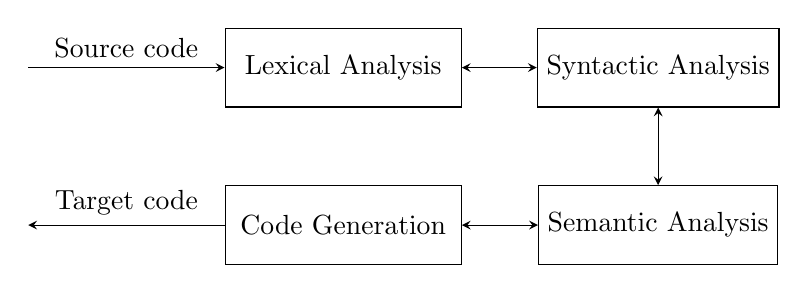
\begin{tikzpicture}[>=stealth, every node/.style={align=center}]

% Nodes
\node[draw, rectangle, minimum width=3cm, minimum height=1cm] (lexical) at (0,0) {Lexical Analysis};
\node[draw, rectangle, minimum width=3cm, minimum height=1cm] (syntactic) at (4,0) {Syntactic Analysis};
\node[draw, rectangle, minimum width=3cm, minimum height=1cm] (semantic) at (4,-2) {Semantic Analysis};
\node[draw, rectangle, minimum width=3cm, minimum height=1cm] (codegen) at (0,-2) {Code Generation};

% Edges
\draw[->] (-4, 0) -- (lexical.west) node[midway, above] {Source code};
\draw[<->] (lexical.east) -- (syntactic.west);
\draw[<->] (syntactic.south) -- (semantic.north);
\draw[<->] (semantic.west) -- (codegen.east);
\draw[->] (codegen.west) -- (-4, -2) node[midway, above] {Target code};

\end{tikzpicture}
\end{document}